\documentclass[polish]{beamer}
\usepackage[T1]{fontenc} % polish characters
\usepackage[polish]{babel} % polish language
\usepackage{graphicx} % images
\usepackage{ragged2e} % justify text
\usepackage{helvet} % font
\usepackage{listings} % code listings
\usepackage{xcolor} % colors
\renewcommand{\familydefault}{\sfdefault}


\usetheme{Warsaw}
\title{Zaprojektowanie i wdrożenie procesu DevOps dla przykładowego systemu oprogramowania}
\author{Sebastian Fudalej}
\institute{Politechnika Opolska}
\date{2023}
% title graphic
\titlegraphic{
\includegraphics[width=0.3\linewidth]{images/logotyp-politechnika-opolska-01.jpg}}

\begin{document}

\frame{\titlepage}

\begin{frame}
    \justifying
    \frametitle{Proces DevOps}
    \begin{figure}
        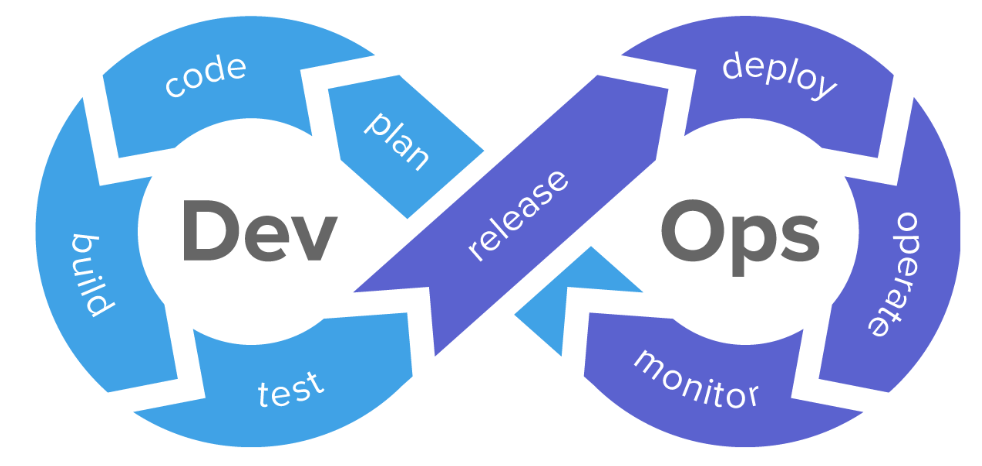
\includegraphics[width=0.5\linewidth]{images/devops.png}
        \caption{DevOps}
        \label{fig:devops}
    \end{figure}
    Proces \textbf{DevOps} to kultura i zestaw praktyk w dziedzinie rozwoju oprogramowania, które łączą działania zespołu programistycznego (Dev) z działaniami związanymi z zarządzaniem infrastrukturą i dostarczaniem aplikacji (Ops).
\end{frame}

\begin{frame}
    \frametitle{Technologie}
    \justifying
    \begin{itemize}
        \item Docker
        \item Jenkins
        \item Ansible
        \item Kubernetes
        \item Git
    \end{itemize}
\end{frame}

\begin{frame}
    \frametitle{Docker}
    \justifying
    \begin{figure}
        
\includegraphics[width=0.5\linewidth]{images/docker_logo.png}
        \caption{Docker}
        \label{fig:docker}
    \end{figure}
    \begin{itemize}
        \item Narzędzie do tworzenia, wdrażania i uruchamiania aplikacji przy użyciu kontenerów
        \item Kontenery są izolowane od siebie i od systemu gospodarza
        \item Kontenery są przenośne i mogą być uruchamiane na dowolnym systemie operacyjnym
    \end{itemize}

\end{frame}


\begin{frame}[fragile]
    \frametitle{Docker Compose}
    Narzędzie do definiowania i uruchamiania wielu kontenerów Docker.
    \newline
    Przykładowy plik \textit{docker-compose.yml}:


    \lstset{
        backgroundcolor=\color{gray!10},
    }

    \begin{lstlisting}
    version: '3.3'
    services:
        web:
            build: .
            ports:
                - "5000:5000"
            environment:
                REDIS_HOST: redis
        redis:
            image: "redis:alpine"
    \end{lstlisting}
\end{frame}

\begin{frame}
    \frametitle{Jenkins}
    \justifying
    \begin{figure}
        
\includegraphics[width=0.5\linewidth]{images/jenkins.png}
        \caption{Jenkins}
        \label{fig:jenkins}
    \end{figure}
    \begin{itemize}
        \item Narzędzie do automatyzacji procesów
        \item Jenkins jest serwerem, który automatyzuje procesy
        \item Jenkins może być używany do automatyzacji wszystkich aspektów tworzenia, testowania i dostarczania oprogramowania
    \end{itemize}
\end{frame}

\begin{frame}
    \frametitle{Wzory matematyczne}
    \begin{equation*}
        a^2 + b^2 = c^2
    \end{equation*}
    \begin{equation*}
        \frac{n!}{k!(n-k)!} = \binom{n}{k}
    \end{equation*}
    \begin{equation*}
        \sum_{i=1}^{n} i = \frac{n(n+1)}{2}
    \end{equation*}
    \begin{equation*}
        \begin{bmatrix}
            1 & 2 & 3 \\
            4 & 5 & 6 \\
            7 & 8 & 9
        \end{bmatrix}
    \end{equation*}
\end{frame}

\begin{frame}[fragile]
    \frametitle{Kod w Pythonie}
    \begin{lstlisting}[language=Python]
        def fib(n):
            a, b = 0, 1
            while a < n:
                print(a, end=' ')
                a, b = b, a+b
            print()
        fib(1000)
    \end{lstlisting}
\end{frame}

\begin{frame}
    \frametitle{Lista numerowana}
    \begin{enumerate}
        \item Pierwszy element
        \item Drugi element
        \item Trzeci element
    \end{enumerate}
    
\end{frame}

\end{document}